\documentclass[11pt,a4paper]{article}

% Encoding and typography
\usepackage[T1]{fontenc}
\usepackage[utf8]{inputenc}
\usepackage{lmodern}
\usepackage{microtype}
\usepackage{amsmath,amssymb}
\usepackage{helvet}
\renewcommand{\familydefault}{\sfdefault}

% Page layout
\usepackage[a4paper,margin=22mm,headheight=23pt]{geometry}
\usepackage{setspace}
\setstretch{1.08}
\usepackage{parskip}
\usepackage{ragged2e}

% Graphics and colour
\usepackage{graphicx}
\usepackage[table]{xcolor}
\usepackage{caption}
\usepackage{subcaption}
\usepackage{float}
\usepackage{tikz}
\usetikzlibrary{arrows.meta,calc,positioning}

% Tables and lists
\usepackage{array}
\usepackage{booktabs}
\usepackage{tabularx}
\usepackage{longtable}
\usepackage{enumitem}
\usepackage{listings}

% Headers, links, and headings
\usepackage{fancyhdr}
\usepackage{lastpage}
\usepackage{titlesec}
\usepackage[most]{tcolorbox}
\usepackage{hyperref}
\usepackage{xurl}

\definecolor{UPBlue}{HTML}{003B5C}
\definecolor{UPAccent}{HTML}{C69214}
\definecolor{UPLight}{HTML}{EEF5F8}
\definecolor{TableHead}{HTML}{DCEAF0}
\definecolor{TableRule}{HTML}{6E8FA3}
\definecolor{CodeBack}{HTML}{F6F8FA}
\definecolor{SolarGreen}{HTML}{2F7D5A}
\definecolor{PanelBlue}{HTML}{2E6F9E}
\definecolor{CoverInk}{HTML}{1B2838}

\hypersetup{
  colorlinks=true,
  linkcolor=UPBlue,
  urlcolor=UPBlue,
  citecolor=UPBlue,
  pdfauthor={Department of Electrical, Electronic and Computer Engineering},
  pdftitle={MPPT Circuit Student Implementation Guide},
  pdfsubject={Module ENR 420},
  pdfkeywords={MPPT, four-switch buck-boost converter, solar panels, STM32, CubeMX}
}
\urlstyle{same}

\graphicspath{{fig/}}
\captionsetup{font=small,labelfont={bf,color=UPBlue},labelsep=colon,skip=4pt}
\renewcommand{\arraystretch}{1.24}
\setlength{\tabcolsep}{6pt}
\newcolumntype{Y}{>{\RaggedRight\arraybackslash}X}
\newcolumntype{L}[1]{>{\raggedright\arraybackslash}p{#1}}
\setlist[itemize]{leftmargin=*,topsep=2pt,itemsep=2pt}
\setlist[enumerate]{leftmargin=*,topsep=2pt,itemsep=2pt}

\lstset{
  basicstyle=\ttfamily\footnotesize,
  backgroundcolor=\color{CodeBack},
  frame=single,
  rulecolor=\color{TableRule},
  breaklines=true,
  columns=fullflexible,
  keepspaces=true,
  showstringspaces=false,
  tabsize=2,
  xleftmargin=1mm,
  xrightmargin=1mm
}

\titleformat{\section}
  {\Large\bfseries\color{UPBlue}}
  {\thesection}{0.65em}{}
\titleformat{\subsection}
  {\large\bfseries\color{UPBlue}}
  {\thesubsection}{0.65em}{}
\titleformat{\subsubsection}
  {\normalsize\bfseries\color{UPBlue}}
  {\thesubsubsection}{0.65em}{}
\titlespacing*{\section}{0pt}{1.2em}{0.55em}
\titlespacing*{\subsection}{0pt}{1.0em}{0.35em}
\titlespacing*{\subsubsection}{0pt}{0.75em}{0.25em}

\pagestyle{fancy}
\fancyhf{}
\lhead{\small MPPT Circuit Student Implementation Guide}
\rhead{\small Module ENR 420}
\cfoot{\small Page \thepage\ of \pageref*{LastPage}}
\renewcommand{\headrulewidth}{0.4pt}
\renewcommand{\headrule}{\hbox to\headwidth{\color{UPAccent}\leaders\hrule height \headrulewidth\hfill}}

\newcommand{\code}[1]{\texttt{#1}}
\newcommand{\Vout}{V_{o}}
\newcommand{\Vin}{V_{\mathrm{in}}}
\newcommand{\Vadc}{V_{\mathrm{ADC}}}
\newcommand{\Vref}{V_{\mathrm{REF}}}
\newcommand{\Pin}{P_{\mathrm{PV}}}
\newcommand{\Iin}{I_{\mathrm{in}}}
\newcommand{\Iout}{I_{\mathrm{o}}}
\newcommand{\Vpv}{V_{\mathrm{PV}}}

\let\originalsection\section
\renewcommand{\section}{\clearpage\originalsection}

\newtcolorbox{guidebox}[1]{
  colback=UPLight,
  colframe=UPBlue,
  boxrule=0.8pt,
  arc=1.5mm,
  left=4mm,right=4mm,top=3mm,bottom=3mm,
  title=\textbf{#1},
  coltitle=white,
  colbacktitle=UPBlue,
  fonttitle=\bfseries
}

\newtcolorbox{warnbox}[1]{
  colback=white,
  colframe=UPAccent,
  boxrule=0.9pt,
  arc=1.5mm,
  left=4mm,right=4mm,top=3mm,bottom=3mm,
  title=\textbf{#1},
  coltitle=black,
  colbacktitle=UPAccent!35,
  fonttitle=\bfseries
}

\begin{document}
\hypersetup{pageanchor=false}
\pagestyle{empty}

% Swap the active cover design by changing this input file.
% Alternatives currently available:
%   title_page_original.tex
%   title_page_blueprint.tex
%   title_page_technical_flow.tex
%   title_page_solar_hero.tex
% \begin{titlepage}
  \thispagestyle{empty}
  \centering
  \vspace*{7mm}
  {\Large\bfseries Department of Electrical, Electronic and Computer Engineering\par}
  \vspace{12mm}
  
\includegraphics[width=0.72\textwidth]{up_logo_transparent.png}\par
  \vspace{16mm}
  {\Huge\bfseries\color{UPBlue} MPPT Circuit Student Implementation Guide\par}
  \vspace{14mm}
  {\LARGE\bfseries Module ENR 420\par}
  \vfill
  \begin{tcolorbox}[
    colback=UPLight,
    colframe=UPBlue,
    width=0.86\textwidth,
    boxrule=0.9pt,
    arc=1.5mm,
    left=5mm,right=5mm,top=4mm,bottom=4mm]
    \centering
    A practical guide to the MPPT circuit, sensing interfaces, gate-driver control, STM32 pin mapping, firmware architecture, and safe laboratory bring-up used in Practicals 1 and 3.
  \end{tcolorbox}
  \vspace*{10mm}
\end{titlepage}

\begin{titlepage}
  \thispagestyle{empty}
  \begin{tikzpicture}[remember picture,overlay]
    \fill[white] (current page.south west) rectangle (current page.north east);

    \begin{scope}
      \clip (current page.north west) rectangle ($(current page.north east)+(0,-176mm)$);
      \node[anchor=north,inner sep=0pt] at (current page.north)
        {
\includegraphics[height=176mm]{solar_hero_cover.png}};
    \end{scope}

    \fill[UPBlue,opacity=0.74] (current page.north west) rectangle ($(current page.north west)+(139mm,-176mm)$);
    \fill[black,opacity=0.16] (current page.north west) rectangle ($(current page.north east)+(0,-176mm)$);
    \fill[UPAccent] ($(current page.north west)+(0,-176mm)$) rectangle ($(current page.north east)+(0,-179mm)$);
    \fill[UPLight] (current page.south west) rectangle ($(current page.south east)+(0,118mm)$);
    \fill[SolarGreen] (current page.south west) rectangle ($(current page.south east)+(0,8mm)$);

    \node[anchor=north west,inner sep=0pt] at ($(current page.north west)+(15mm,-10mm)$)
      {
\includegraphics[width=0.30\paperwidth]{up_logo_white_transparent.png}};
    \node[anchor=north east,align=right,text=white,font=\bfseries\normalsize] at ($(current page.north east)+(-15mm,-13mm)$)
      {Department of Electrical, Electronic\\and Computer Engineering};

    \node[anchor=north west,align=left,text width=0.60\paperwidth] at ($(current page.north west)+(17mm,-57mm)$)
      {{\color{UPAccent}\rule{24mm}{1.2pt}}\par
       \vspace{4mm}
       {\fontsize{29}{34}\selectfont\bfseries\color{white} MPPT Circuit\\Student Implementation\\Guide\par}
       \vspace{6mm}
       {\Large\bfseries\color{white} Module ENR 420\par}
       };

    \node[anchor=north west,align=left,text width=0.64\paperwidth] at ($(current page.south west)+(22mm,101mm)$)
      {{\large\bfseries\color{UPBlue} Photovoltaic maximum power point tracking\\for safe laboratory implementation\par}
       \vspace{3mm}
       {\normalsize\color{CoverInk} A practical guide to the MPPT circuit, sensing interfaces, gate\mbox{-}driver control, STM32 pin mapping, firmware architecture, and safe laboratory bring-up used in Practicals 1 and 3.\par}};

    \node[anchor=north east,align=center] at ($(current page.south east)+(-24mm,101mm)$)
      {\begin{tikzpicture}[
        small/.style={draw=UPBlue!70,fill=white,rounded corners=1mm,minimum width=24mm,minimum height=8mm,align=center,font=\scriptsize\bfseries},
        arrow/.style={-{Latex[length=1.8mm]},draw=UPAccent,line width=0.65pt}
      ]
        \node[small,fill=PanelBlue!10] (pv) {PV input};
        \node[small,below=5mm of pv] (conv) {MPPT};
        \node[small,fill=SolarGreen!12,below=5mm of conv] (load) {Load};
        \draw[arrow] (pv) -- (conv);
        \draw[arrow] (conv) -- (load);
      \end{tikzpicture}};

    \draw[UPBlue!35,line width=0.8pt] ($(current page.south west)+(22mm,41mm)$) -- ($(current page.south east)+(-22mm,41mm)$);
    \node[anchor=south,align=center,text=UPBlue,font=\small\bfseries] at ($(current page.south)+(0,20mm)$)
      {solar energy management \textbar{} power conversion \textbar{} embedded control};
  \end{tikzpicture}
\end{titlepage}

% \begin{titlepage}
  \thispagestyle{empty}
  \begin{tikzpicture}[remember picture,overlay]
    \fill[white] (current page.south west) rectangle (current page.north east);
    \fill[UPLight] (current page.south west) rectangle ($(current page.south east)+(0,42mm)$);
    \fill[UPBlue] (current page.north west) rectangle ($(current page.north east)+(0,-26mm)$);
    \fill[UPAccent] ($(current page.north west)+(0,-26mm)$) rectangle ($(current page.north east)+(0,-28mm)$);

    \foreach \y in {48,58,...,246}
      \draw[TableRule!12,line width=0.2pt] ($(current page.south west)+(0,\y mm)$) -- ($(current page.south east)+(0,\y mm)$);
    \foreach \x in {16,28,...,194}
      \draw[TableRule!10,line width=0.2pt] ($(current page.south west)+(\x mm,42mm)$) -- ($(current page.north west)+(\x mm,-34mm)$);

    \node[anchor=north west,inner sep=0pt] at ($(current page.north west)+(14mm,-8mm)$)
      {
\includegraphics[width=0.29\paperwidth]{up_logo_white_transparent.png}};
    \node[anchor=north east,align=right,text=white,font=\bfseries\large] at ($(current page.north east)+(-14mm,-10mm)$)
      {Department of Electrical, Electronic\\and Computer Engineering};

    \draw[UPBlue!35,line width=0.8pt] ($(current page.north west)+(14mm,-42mm)$) -- ($(current page.north east)+(-14mm,-42mm)$);
    \draw[UPAccent,line width=1.0pt] ($(current page.north west)+(14mm,-58mm)$) -- ($(current page.north west)+(44mm,-58mm)$);

    \node[anchor=south east,opacity=0.10] at ($(current page.south east)+(-8mm,50mm)$)
      {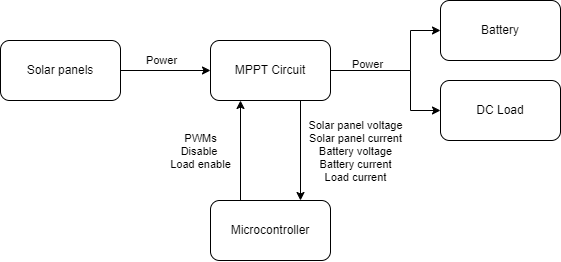
\includegraphics[width=0.52\paperwidth]{system_block_diagram.png}};
  \end{tikzpicture}

  \vspace*{52mm}
  \noindent
  {\fontsize{30}{35}\selectfont\bfseries\color{UPBlue} MPPT Circuit Student\\Implementation Guide\par}
  \vspace{5mm}
  {\Large\bfseries\color{CoverInk} Module ENR 420\par}

  \vspace{14mm}
  \begin{center}
    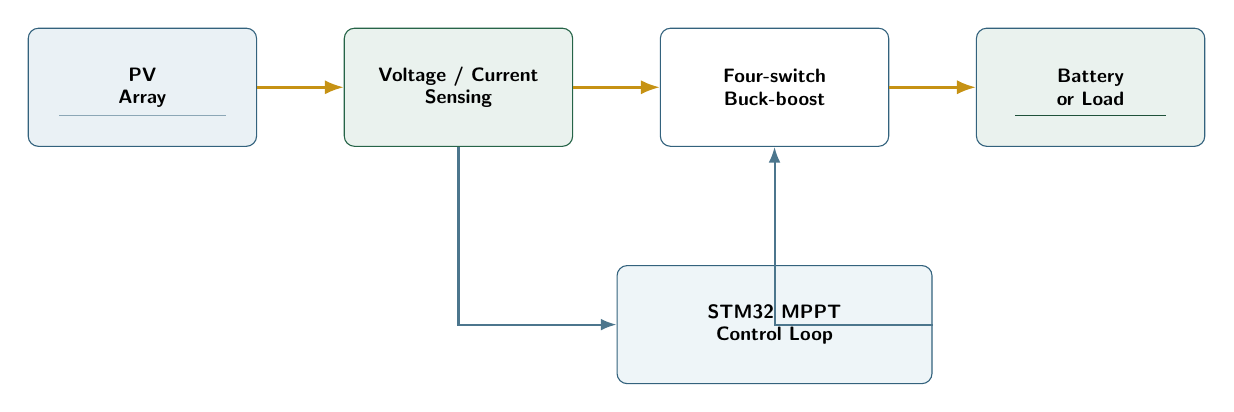
\begin{tikzpicture}[
      module/.style={draw=UPBlue!80,fill=white,rounded corners=1.3mm,minimum width=29mm,minimum height=15mm,align=center,font=\scriptsize\bfseries},
      sensor/.style={draw=SolarGreen!80!black,fill=SolarGreen!10,rounded corners=1.3mm,minimum width=29mm,minimum height=15mm,align=center,font=\scriptsize\bfseries},
      arrow/.style={-{Latex[length=2.4mm]},draw=UPAccent,line width=0.9pt},
      loop/.style={-{Latex[length=2.0mm]},draw=UPBlue!70,line width=0.75pt}
    ]
      \node[module,fill=PanelBlue!10] (pv) {PV\\Array};
      \node[sensor,right=11mm of pv] (sense) {Voltage / Current\\Sensing};
      \node[module,right=11mm of sense] (conv) {Four-switch\\Buck-boost};
      \node[module,fill=SolarGreen!10,right=11mm of conv] (load) {Battery\\or Load};
      \node[module,fill=UPLight,below=15mm of conv,minimum width=40mm] (ctrl) {STM32 MPPT\\Control Loop};

      \draw[arrow] (pv) -- (sense);
      \draw[arrow] (sense) -- (conv);
      \draw[arrow] (conv) -- (load);
      \draw[loop] (sense.south) |- (ctrl.west);
      \draw[loop] (ctrl.east) -| (conv.south);

      \draw[UPBlue!45,line width=0.45pt] ($(pv.south west)+(4mm,4mm)$) -- ($(pv.south east)+(-4mm,4mm)$);
      \draw[SolarGreen!65!black,line width=0.55pt] ($(load.south west)+(5mm,4mm)$) -- ($(load.south east)+(-5mm,4mm)$);
    \end{tikzpicture}
  \end{center}

  \vfill
  \begin{tcolorbox}[
    enhanced,
    colback=UPLight,
    colframe=UPBlue,
    width=\textwidth,
    boxrule=0.9pt,
    arc=1.2mm,
    left=5mm,right=5mm,top=4mm,bottom=4mm,
    borderline west={2.4pt}{0pt}{UPAccent}]
    \large
    A practical guide to the MPPT circuit, sensing interfaces, gate-driver control, STM32 pin mapping, firmware architecture, and safe laboratory bring-up used in Practicals 1 and 3.
  \end{tcolorbox}

  \vspace{8mm}
  \begin{center}
    {\small\bfseries\color{UPBlue} Photovoltaic input \textbar{} measured power \textbar{} converter command \textbar{} safe embedded control}
  \end{center}
  \vspace*{4mm}
\end{titlepage}

% \begin{titlepage}
  \thispagestyle{empty}
  \begin{tikzpicture}[remember picture,overlay]
    \fill[UPLight] (current page.south west) rectangle (current page.north east);

    \foreach \x in {0,8,...,216}
      \draw[TableRule!16,line width=0.2pt] ($(current page.south west)+(\x mm,0)$) -- ($(current page.north west)+(\x mm,0)$);
    \foreach \y in {0,8,...,304}
      \draw[TableRule!16,line width=0.2pt] ($(current page.south west)+(0,\y mm)$) -- ($(current page.south east)+(0,\y mm)$);

    \fill[UPBlue] (current page.north west) rectangle ($(current page.north east)+(0,-31mm)$);
    \fill[UPAccent] ($(current page.north west)+(0,-31mm)$) rectangle ($(current page.north east)+(0,-33mm)$);
    \fill[SolarGreen] ($(current page.south west)+(0,0)$) rectangle ($(current page.south east)+(0,8mm)$);

    \node[opacity=0.055,anchor=center] at ($(current page.center)+(30mm,-8mm)$)
      {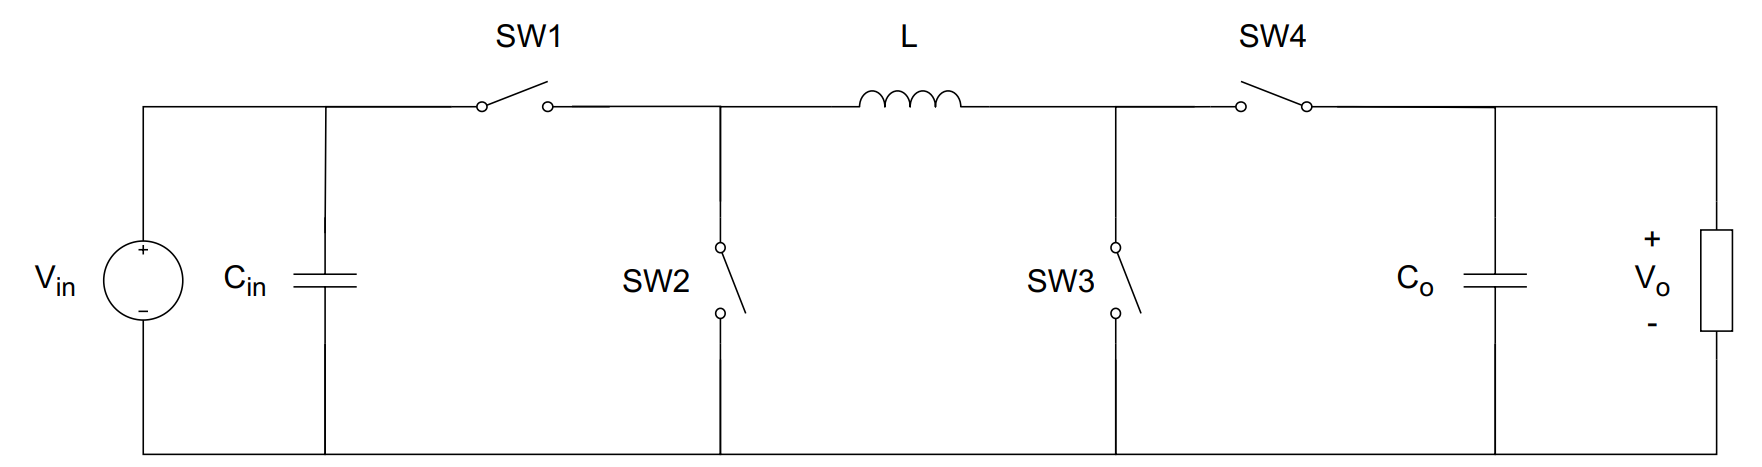
\includegraphics[width=0.92\paperwidth]{four_switch_buck_boost.png}};
    \node[opacity=0.055,anchor=south east] at ($(current page.south east)+(-17mm,40mm)$)
      {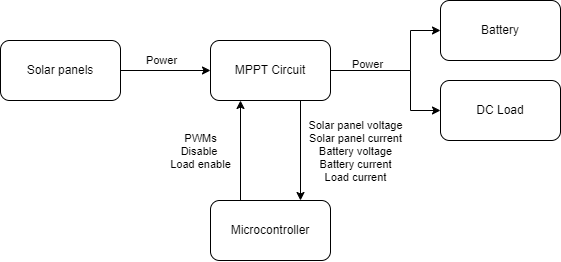
\includegraphics[width=0.36\paperwidth]{system_block_diagram.png}};

    \draw[UPBlue!38,line width=0.7pt] ($(current page.north west)+(14mm,-45mm)$) -- ($(current page.north east)+(-14mm,-45mm)$);
    \draw[UPBlue!38,line width=0.7pt] ($(current page.south west)+(14mm,48mm)$) -- ($(current page.south east)+(-14mm,48mm)$);

    \node[anchor=north west,inner sep=0pt] at ($(current page.north west)+(14mm,-7mm)$)
      {
\includegraphics[height=17mm]{up_logo_white_transparent.png}};
    \node[anchor=north east,align=right,text=white,font=\bfseries\normalsize] at ($(current page.north east)+(-15mm,-10mm)$)
      {Department of Electrical, Electronic\\and Computer Engineering};
  \end{tikzpicture}

  \vspace*{49mm}
  \noindent
  \begin{minipage}[t]{0.61\textwidth}
    {\color{UPAccent}\rule{22mm}{1.2pt}\par}
    \vspace{4mm}
    {\fontsize{29}{34}\selectfont\bfseries\color{UPBlue} MPPT Circuit\\Student Implementation\\Guide\par}
    \vspace{5mm}
    {\Large\bfseries\color{CoverInk} Module ENR 420\par}
  \end{minipage}\hfill
  \begin{minipage}[t]{0.31\textwidth}
    \vspace{11mm}
    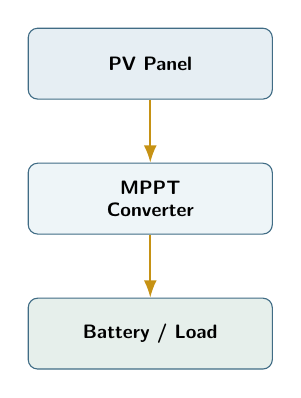
\begin{tikzpicture}[
      node distance=8mm,
      flow/.style={draw=UPBlue!75,fill=white,rounded corners=1.2mm,minimum width=31mm,minimum height=9mm,align=center,font=\scriptsize\bfseries},
      arrow/.style={-{Latex[length=2.2mm]},line width=0.7pt,draw=UPAccent}
    ]
      \node[flow,fill=PanelBlue!12] (pv) {PV Panel};
      \node[flow,below=of pv,fill=UPLight] (mppt) {MPPT\\Converter};
      \node[flow,below=of mppt,fill=SolarGreen!12] (load) {Battery / Load};
      \draw[arrow] (pv) -- (mppt);
      \draw[arrow] (mppt) -- (load);
    \end{tikzpicture}
  \end{minipage}

  \vfill
  \begin{center}
  \begin{tcolorbox}[
    enhanced,
    colback=white,
    colframe=UPBlue,
    width=0.88\textwidth,
    boxrule=0.9pt,
    arc=1.2mm,
    left=5mm,right=5mm,top=4mm,bottom=4mm,
    borderline west={2.4pt}{0pt}{UPAccent}]
    \RaggedRight\normalsize
    A practical guide to the MPPT circuit, sensing interfaces, gate-driver control, STM32 pin mapping, firmware architecture, and safe laboratory bring-up used in Practicals 1 and 3.
  \end{tcolorbox}
  \end{center}

  \vspace{8mm}
  \begin{center}
    {\small\bfseries\color{UPBlue} Photovoltaic energy management \textbar{} power conversion \textbar{} embedded control}
  \end{center}
  \vspace*{2mm}
\end{titlepage}


\thispagestyle{empty}
\tableofcontents
\clearpage
\hypersetup{pageanchor=true}
\pagenumbering{arabic}
\pagestyle{fancy}

\section{How This Guide Should Be Used}

Welcome to your final-year power electronics project! If your previous experience was writing a basic PID controller on a microcontroller, this project is a fantastic step up. You are going to build the brain for a custom power electronics converter to extract the maximum possible power from solar panels.

This guide provides the system architecture, equations, hardware specifics, and printed circuit board (PCB) layouts you need to program the \href{https://www.st.com/en/evaluation-tools/nucleo-f303k8.html}{STM32 NUCLEO-F303K8} microcontroller. \textit{However, it is not a finished solution.} The exact timing, control algorithms, digital filtering, and data parsing will rely on your engineering judgment to bridge the gaps.

\begin{guidebox}{Learning outcomes}
After working through this guide you should be able to:
\begin{itemize}
  \item explain how the four-switch buck-boost converter changes the solar-panel operating point;
  \item identify each PCB signal connected to the STM32 and configure the matching GPIO, ADC, UART, and timer peripherals;
  \item convert raw ADC counts into real-world voltage, current, power, and irradiance values;
  \item design a robust state machine that starts safely, checks measurements, limits duty cycles, and handles faults;
  \item communicate with digital sensors and your PC over serial protocols;
  \item verify the firmware in the laboratory before connecting the full solar-panel and battery system.
\end{itemize}
\end{guidebox}

\subsection{Assumed background}

You are expected to know the basic operation of DC-DC converters, MOSFET switching, PWM, ADC sampling, UART communication, and C programming. The guide fills in the project-specific details: which signals exist on this PCB, how the sensor outputs relate to physical units, and how the STM32 firmware should be organised.

\begin{warnbox}{Safe laboratory sequence}
Do not connect the solar panels, battery, or load during first firmware testing. First confirm that the STM32 boots, the gate-driver disable pins keep switching disabled, ADC readings are plausible, and PWM waveforms are correct on an oscilloscope. Only then proceed to current-limited converter testing.
\end{warnbox}

\section{System Overview}

Solar panels are highly non-linear; their power output changes depending on how much current you draw from them. If you draw too little, voltage is high but current is near zero (no power). If you draw too much, voltage collapses to zero (no power). 

Your goal is to find the "sweet spot" in the middle: the \textbf{Maximum Power Point (MPPT)}.

Because you cannot control the sun, you control the \textbf{duty cycle} of a DC-DC converter. By changing the duty cycle, you change the "electrical resistance" the solar panel sees, which shifts its operating voltage and current. The MPPT algorithm observes the resulting panel voltage and current, estimates $\Pin=\Vpv\Iin$, and adjusts the converter command until the operating point is close to the peak.

Figure~\ref{fig:system-block-diagram} shows the complete system with the PV input, measurement feedback, MPPT controller, PWM/gate-driver path, and four-switch buck-boost power stage. The MPPT PCB draws power from two series-connected \href{https://www.offgridtec.com/media/product_attachements/YingliSolar_410W\%20YLM-J\%203.0\%20PRO_Datasheet.pdf}{Yingli YLM-J 3.0 PRO solar panels} and delivers power to the output terminals. 

\begin{figure}[H]
  \centering
  \resizebox{\textwidth}{!}{%
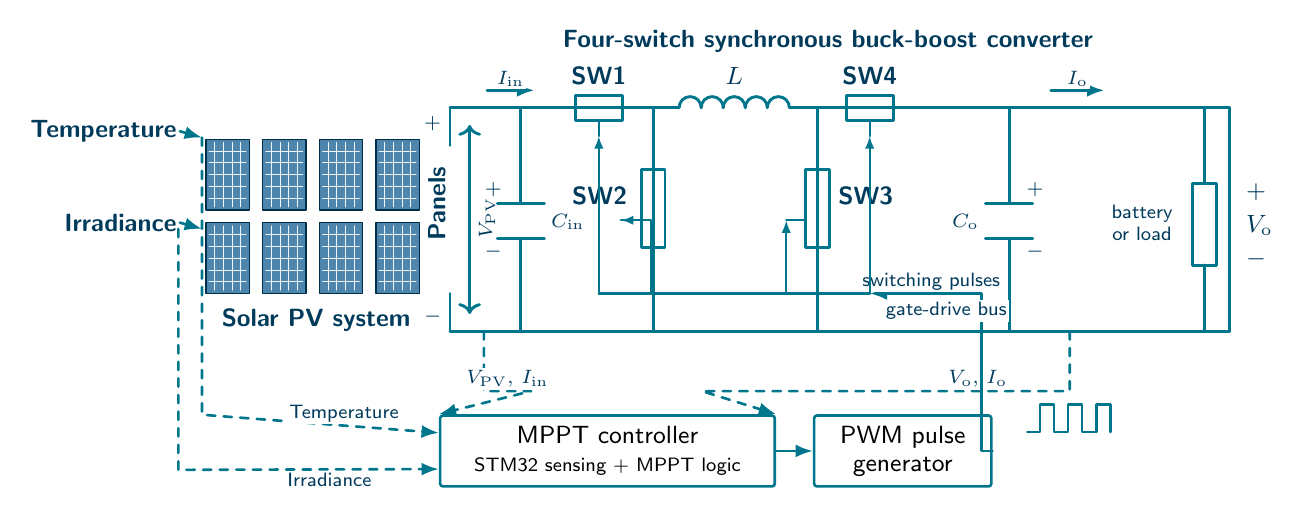
\begin{tikzpicture}[
  x=1cm,
  y=1cm,
  line cap=round,
  line join=round,
  wire/.style={draw=UPBlue!70!cyan, line width=1.05pt},
  flow/.style={draw=UPBlue!70!cyan, line width=0.95pt, -{Latex[length=2.2mm]}},
  sense/.style={draw=UPBlue!70!cyan, line width=0.95pt, dashed, -{Latex[length=2.2mm]}},
  signal/.style={draw=UPBlue!70!cyan, line width=0.85pt},
  block/.style={draw=UPBlue!70!cyan, fill=white, line width=0.95pt, rounded corners=1pt, align=center, font=\small},
  label/.style={font=\small\bfseries, text=UPBlue, fill=white, inner sep=1pt},
  smalllabel/.style={font=\scriptsize, text=UPBlue, fill=white, inner sep=0.8pt}
]

% Solar PV array, arranged to match the left-hand panel bank in the reference.
\foreach \r in {0,1} {
  \foreach \c in {0,1,2,3} {
    \begin{scope}[shift={(1.35+0.72*\c,2.72+1.06*\r)}]
      \draw[draw=UPBlue!80!black, fill=PanelBlue!85, line width=0.45pt] (0,0) rectangle (0.55,0.90);
      \foreach \gx in {0.11,0.22,0.33,0.44} {
        \draw[UPLight, line width=0.22pt] (\gx,0.04) -- (\gx,0.86);
      }
      \foreach \gy in {0.15,0.30,0.45,0.60,0.75} {
        \draw[UPLight, line width=0.22pt] (0.04,\gy) -- (0.51,\gy);
      }
    \end{scope}
  }
}
\node[label] at (2.75,2.38) {Solar PV system};
\node[label, rotate=90] at (4.28,3.86) {Panels};

% Environmental inputs to the panel side.
\node[label, anchor=east] (temp) at (1.02,4.78) {Temperature};
\node[label, anchor=east] (irr) at (1.02,3.62) {Irradiance};
\draw[flow] (temp.east) -- (1.30,4.70);
\draw[flow] (irr.east) -- (1.30,3.54);

% Power rails: PV array into the four-switch buck-boost stage.
% The positive path is intentionally broken by the controlled switches and inductor
% so the 4SBB topology is not shown as a continuous shorted rail.
\draw[wire] (4.45,5.08) -- (5.78,5.08);
\draw[wire] (4.45,2.24) -- (14.35,2.24);
\draw[wire] (4.45,5.08) -- (4.45,4.60);
\draw[wire] (4.45,2.24) -- (4.45,2.72);
\node[smalllabel] at (4.23,4.88) {$+$};
\node[smalllabel] at (4.23,2.42) {$-$};
\draw[wire,<->] (4.70,4.86) -- (4.70,2.46);
\node[smalllabel, rotate=90] at (4.92,3.68) {$V_{\mathrm{PV}}$};
\draw[flow] (4.92,5.30) -- node[smalllabel, above] {$I_{\mathrm{in}}$} (5.52,5.30);

% Input capacitor.
\draw[wire] (5.35,5.08) -- (5.35,3.86);
\draw[wire] (5.05,3.86) -- (5.65,3.86);
\draw[wire] (5.05,3.42) -- (5.65,3.42);
\draw[wire] (5.35,3.42) -- (5.35,2.24);
\node[smalllabel, right] at (5.70,3.63) {$C_{\mathrm{in}}$};
\node[smalllabel] at (5.00,4.04) {$+$};
\node[smalllabel] at (5.00,3.25) {$-$};

% Buck-side high switch, SW1.
\draw[wire] (5.78,5.08) -- (6.04,5.08);
\draw[wire, fill=white] (6.04,4.92) rectangle (6.64,5.24);
\draw[wire] (6.04,5.08) -- (6.64,5.08);
\draw[signal] (6.34,4.72) -- (6.34,4.92);
\draw[wire] (6.64,5.08) -- (7.03,5.08);
\node[label] at (6.34,5.48) {SW1};

% Buck-side low switch, SW2.
\draw[wire] (7.03,5.08) -- (7.03,4.30);
\draw[wire, fill=white] (6.88,3.30) rectangle (7.18,4.30);
\draw[wire] (7.03,4.30) -- (7.03,3.30);
\draw[signal] (6.62,3.65) -- (6.88,3.65);
\draw[wire] (7.03,3.30) -- (7.03,2.24);
\node[label, anchor=east] at (6.74,3.96) {SW2};

% Inductor between the buck and boost switching nodes.
\draw[wire] (7.03,5.08) -- (7.36,5.08);
\foreach \x in {7.36,7.64,7.92,8.20,8.48} {
  \draw[wire] (\x,5.08) arc[start angle=180, end angle=0, radius=0.14];
}
\draw[wire] (8.76,5.08) -- (9.12,5.08);
\node[label] at (8.06,5.48) {$L$};

% Boost-side low switch, SW3.
\draw[wire] (9.12,5.08) -- (9.12,4.30);
\draw[wire, fill=white] (8.97,3.30) rectangle (9.27,4.30);
\draw[wire] (9.12,4.30) -- (9.12,3.30);
\draw[signal] (8.72,3.65) -- (8.97,3.65);
\draw[wire] (9.12,3.30) -- (9.12,2.24);
\node[label, anchor=west] at (9.34,3.96) {SW3};

% Boost-side high switch, SW4.
\draw[wire] (9.12,5.08) -- (9.48,5.08);
\draw[wire, fill=white] (9.48,4.92) rectangle (10.08,5.24);
\draw[wire] (9.48,5.08) -- (10.08,5.08);
\draw[signal] (9.78,4.72) -- (9.78,4.92);
\draw[wire] (10.08,5.08) -- (14.35,5.08);
\node[label] at (9.78,5.48) {SW4};

% Output capacitor and load/battery terminal.
\draw[wire] (11.55,5.08) -- (11.55,3.86);
\draw[wire] (11.25,3.86) -- (11.85,3.86);
\draw[wire] (11.25,3.42) -- (11.85,3.42);
\draw[wire] (11.55,3.42) -- (11.55,2.24);
\node[smalllabel, left] at (11.20,3.63) {$C_{\mathrm{o}}$};
\node[smalllabel] at (11.88,4.04) {$+$};
\node[smalllabel] at (11.88,3.25) {$-$};

\draw[wire] (14.35,5.08) -- (14.35,2.24);
\draw[wire, fill=white] (13.88,3.08) rectangle (14.18,4.12);
\draw[wire] (14.03,5.08) -- (14.03,4.12);
\draw[wire] (14.03,3.08) -- (14.03,2.24);
\node[smalllabel, align=center] at (13.24,3.62) {battery\\or load};
\node[label, anchor=west] at (14.52,4.00) {$+$};
\node[label, anchor=west] at (14.52,3.58) {$V_{\mathrm{o}}$};
\node[label, anchor=west] at (14.52,3.16) {$-$};
\draw[flow] (12.08,5.30) -- node[smalllabel, above] {$I_{\mathrm{o}}$} (12.76,5.30);

% Controller and PWM generator blocks under the power circuit.
\node[block, minimum width=4.25cm, minimum height=0.90cm] (controller) at (6.45,0.72)
  {MPPT controller\\[-1pt]\scriptsize STM32 sensing + MPPT logic};
\node[block, minimum width=2.25cm, minimum height=0.90cm] (pwm) at (10.20,0.72)
  {PWM pulse\\[-1pt]generator};
\draw[flow] (controller.east) -- (pwm.west);

% Feedback paths, styled like the dashed paths in the reference.
\draw[sense] (1.30,4.70) -- (1.30,1.18) -- node[smalllabel, above, pos=0.60] {Temperature} ([yshift=0.23cm]controller.west);
\draw[sense] (1.00,3.54) -- (1.00,0.48) -- node[smalllabel, below, pos=0.58] {Irradiance} ([yshift=-0.23cm]controller.west);

\draw[sense] (4.88,2.24) -- (4.88,1.48) --
  node[smalllabel, above] {$V_{\mathrm{PV}},\,I_{\mathrm{in}}$} (5.48,1.48) -- (controller.north west);
\draw[sense] (12.32,2.24) -- (12.32,1.48) --
  node[smalllabel, above, pos=0.25] {$V_{\mathrm{o}},\,I_{\mathrm{o}}$} (7.65,1.48) -- (controller.north east);

% PWM signal path into the converter: a common gate-drive bus with branches to
% each controlled switch, making the switching-pulse direction unambiguous.
\draw[flow] (pwm.east) -- (11.20,0.72) -- (11.20,2.72) --
  node[smalllabel, above, pos=0.45] {switching pulses} (9.78,2.72);
\draw[signal] (9.78,2.72) -- (6.34,2.72);
\draw[signal,-{Latex[length=1.6mm]}] (6.34,2.72) -- (6.34,4.72);
\draw[signal,-{Latex[length=1.6mm]}] (7.00,2.72) -- (7.00,3.65) -- (6.62,3.65);
\draw[signal,-{Latex[length=1.6mm]}] (8.72,2.72) -- (8.72,3.65);
\draw[signal,-{Latex[length=1.6mm]}] (9.78,2.72) -- (9.78,4.72);
\node[smalllabel, anchor=west] at (9.95,2.50) {gate-drive bus};

% Pulse train icon next to the PWM generator, as in the reference figure.
\draw[UPBlue!70!cyan, line width=0.85pt]
  (11.78,0.96) -- (11.94,0.96) -- (11.94,1.31) -- (12.12,1.31) --
  (12.12,0.96) -- (12.30,0.96) -- (12.30,1.31) -- (12.48,1.31) --
  (12.48,0.96) -- (12.66,0.96) -- (12.66,1.31) -- (12.84,1.31) --
  (12.84,0.96);

\node[label] at (9.25,5.92) {Four-switch synchronous buck-boost converter};
\end{tikzpicture}%
}

  \caption{MPPT system diagram with four-switch buck-boost converter}
  \label{fig:system-block-diagram}
\end{figure}

\begin{guidebox}{Control objective}
For Practical 3, the controller should search for the PV operating point that gives the highest measured input power, $\Pin=\Vpv\Iin$, while keeping converter voltage, current, duty cycle, temperature, and communication conditions inside safe limits.
\end{guidebox}

\section{Circuit Description}

\subsection{Four-switch buck-boost converter}

The DC-DC converter is a four-switch buck-boost (4SBB) converter. Because solar voltage fluctuates depending on irradiance and temperature (and your battery/load voltage varies), the 4SBB allows you to step the input voltage down or up without inverting the output polarity.

\begin{figure}[H]
  \centering
  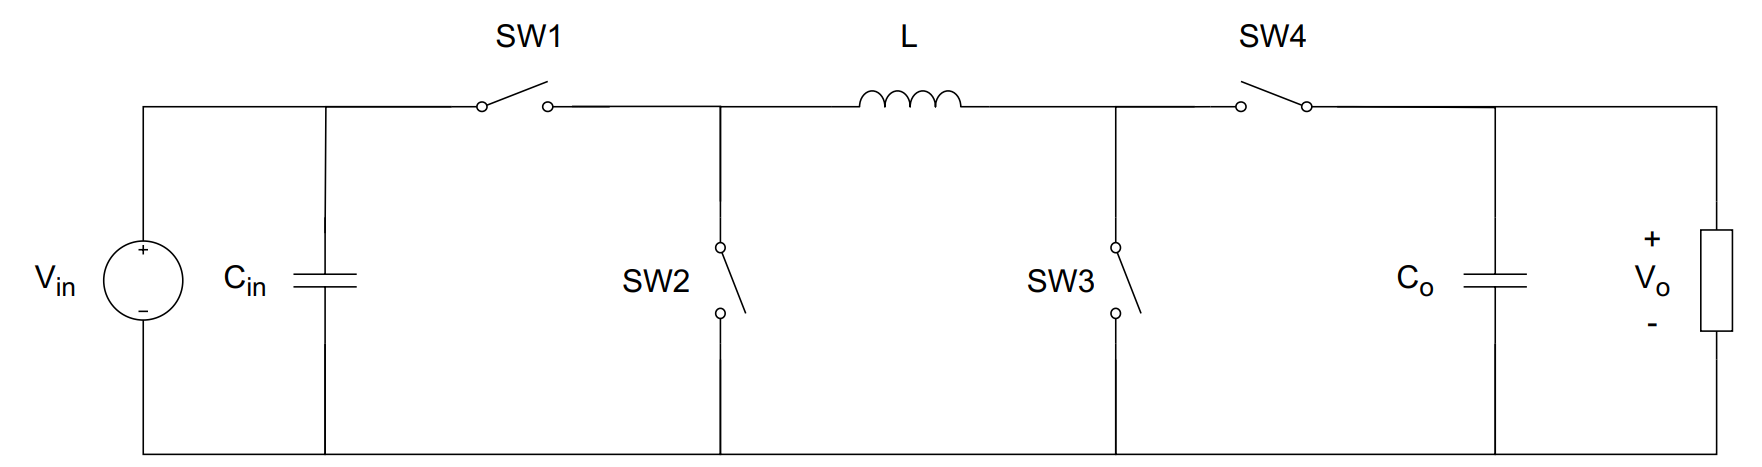
\includegraphics[width=\textwidth]{four_switch_buck_boost.png}
  \caption{Four-switch buck-boost converter circuit diagram}
  \label{fig:four-switch-buck-boost}
\end{figure}

SW1 and SW2 form the buck half bridge. SW3 and SW4 form the boost half bridge. The inductor transfers energy between the input side and the output side. The input and output capacitors reduce switching ripple and provide local energy storage.

Switch 1 and switch 2 operate with complementary duty cycles of $D_1$ and $1-D_1$. Switch 3 and switch 4 operate with duty cycles of $D_2$ and $1-D_2$. The ideal continuous-conduction voltage gain is
\begin{equation}
  \frac{\Vout}{\Vin}=\frac{D_1}{1-D_2}.
  \label{eq:voltage-gain}
\end{equation}

The useful operating cases are:
\begin{itemize}
  \item \textbf{Buck mode}: set $D_2=0$. SW4 remains on, SW3 remains off, and the gain is approximately $D_1$.
  \item \textbf{Boost mode}: set $D_1=1$. SW1 remains on, SW2 remains off, and the gain is approximately $1/(1-D_2)$.
  \item \textbf{Buck-boost mode}: set both sides to switch, for example $D_1=D_2=D$, giving a gain of approximately $D/(1-D)$.
\end{itemize}

The firmware should not jump directly between extreme duty cycles. Use limited duty-cycle ranges, ramp commands gradually during startup, and stop switching immediately when a fault is detected. 

\subsection{Ratings and component values}

The maximum ratings of the circuit are given in Table~\ref{tab:max-ratings}. These are hardware limits, not firmware targets. The controller must operate below these values and should include a safety margin.

\begin{table}[H]
  \centering
  \caption{Circuit maximum ratings}
  \label{tab:max-ratings}
  \begin{tabularx}{0.70\textwidth}{@{}Y r@{}}
    \toprule
    \rowcolor{TableHead}\textbf{Parameter} & \textbf{Value} \\
    \midrule
    Input voltage  & $100\,\mathrm{V}$ \\
    Input current  & $15\,\mathrm{A}$ \\
    Output voltage & $60\,\mathrm{V}$ \\
    Output current & $25\,\mathrm{A}$ \\
    \bottomrule
  \end{tabularx}
\end{table}

The component values used for the inductor and capacitors are given in Table~\ref{tab:component-values}. The circuit is designed for a switching frequency of $250\,\mathrm{kHz}$.

\begin{table}[H]
  \centering
  \caption{Component values}
  \label{tab:component-values}
  \begin{tabularx}{0.70\textwidth}{@{}Y r@{}}
    \toprule
    \rowcolor{TableHead}\textbf{Parameter} & \textbf{Value} \\
    \midrule
    $C_{\mathrm{in}}$ & $25\,\mu\mathrm{F}$ \\
    $L$               & $20\,\mu\mathrm{H}$ \\
    $C_o$             & $15\,\mu\mathrm{F}$ \\
    \bottomrule
  \end{tabularx}
\end{table}

At $250\,\mathrm{kHz}$, one PWM period is
\begin{equation}
  T_s=\frac{1}{250\,000}=4\,\mu\mathrm{s}.
\end{equation}
The commanded duty cycles therefore change the relative on-time of MOSFETs within a $4\,\mu\mathrm{s}$ switching period. 

\section{Safety and Operating Envelope}

The practical system can involve high DC voltage, high current, large capacitors, a battery, and outdoor PV panels. Firmware errors can therefore damage hardware. The first goal of the firmware is safe control. MPPT performance comes after safe startup, measurement sanity checks, and fault handling.

\subsection{Panel operating expectations}

Two series-connected YLM-J 3.0 PRO modules can produce an open-circuit voltage in the region of twice the single-module open-circuit voltage. A typical YLM-J 3.0 PRO 390--415 W module has $V_{\mathrm{MPP}}$ around $30$--$31\,\mathrm{V}$, $I_{\mathrm{MPP}}$ around $13\,\mathrm{A}$, and $V_{\mathrm{OC}}$ around $37\,\mathrm{V}$ at standard test conditions. Two modules in series therefore place the expected maximum-power voltage near $60$--$62\,\mathrm{V}$ and open-circuit voltage near $74\,\mathrm{V}$ before temperature corrections. This is below the PCB input-voltage rating, but it is still hazardous and must be treated as a high-energy DC source.

\subsection{Firmware fault limits}

Use conservative limits in early tests. The values in Table~\ref{tab:fault-limits} are suggested starting limits for firmware development and should be confirmed by the demonstrator for the final practical setup.

\begin{table}[H]
  \centering
  \caption{Suggested firmware fault limits for bring-up}
  \label{tab:fault-limits}
  \begin{tabularx}{\textwidth}{@{}L{0.23\textwidth} L{0.22\textwidth} Y@{}}
    \toprule
    \rowcolor{TableHead}\textbf{Quantity} & \textbf{Initial action limit} & \textbf{Firmware action} \\
    \midrule
    Input voltage & Below hardware rating with margin & Disable PWM if the measured value exceeds the approved practical limit. \\
    Input current & Current-limited during first tests & Disable PWM and log a fault if the input current rises unexpectedly. \\
    Output voltage & Below battery/load rating & Disable PWM if output voltage is too high or inconsistent with the load. \\
    Output current & Below practical limit & Disable PWM on overcurrent or negative current if not expected by the test. \\
    Duty cycle & Keep away from 0\% and 100\% & Clamp commands and ramp slowly. \\
    Sensor validity & ADC and UART values plausible & Do not run MPPT from invalid measurements. \\
    \bottomrule
  \end{tabularx}
\end{table}

\section{Printed Circuit Board Configuration}

A printed circuit board (PCB) has been designed and manufactured for the MPPT circuit. The circuit includes the converter, voltage sensors, current sensors, auxiliary power supplies, gate drivers, microcontroller headers, and irradiance-sensor interface. The unpopulated PCB is shown in Figures~\ref{fig:pcb-unpop-top} and~\ref{fig:pcb-unpop-bottom}.

\begin{figure}[H]
  \centering
  \begin{minipage}[t]{0.47\textwidth}
    \centering
    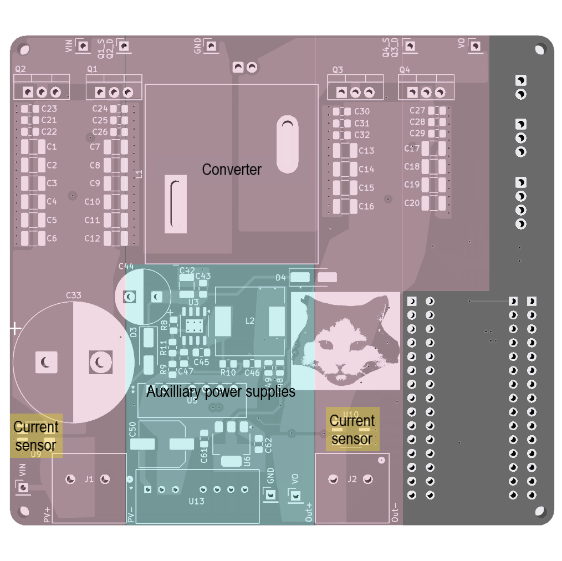
\includegraphics[width=0.92\linewidth]{pcb_unpopulated_top.png}
    \caption{Unpopulated PCB top view}
    \label{fig:pcb-unpop-top}
  \end{minipage}\hfill
  \begin{minipage}[t]{0.47\textwidth}
    \centering
    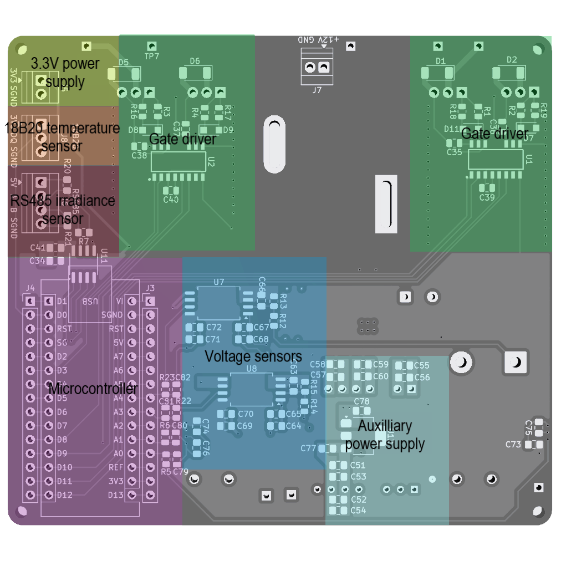
\includegraphics[width=0.92\linewidth]{pcb_unpopulated_bottom.png}
    \caption{Unpopulated PCB bottom view}
    \label{fig:pcb-unpop-bottom}
  \end{minipage}
\end{figure}

The PCB is pictured with components in Figures~\ref{fig:pcb-top-components} and~\ref{fig:pcb-bottom-components}.

\begin{figure}[H]
  \centering
  \begin{minipage}[t]{0.47\textwidth}
    \centering
    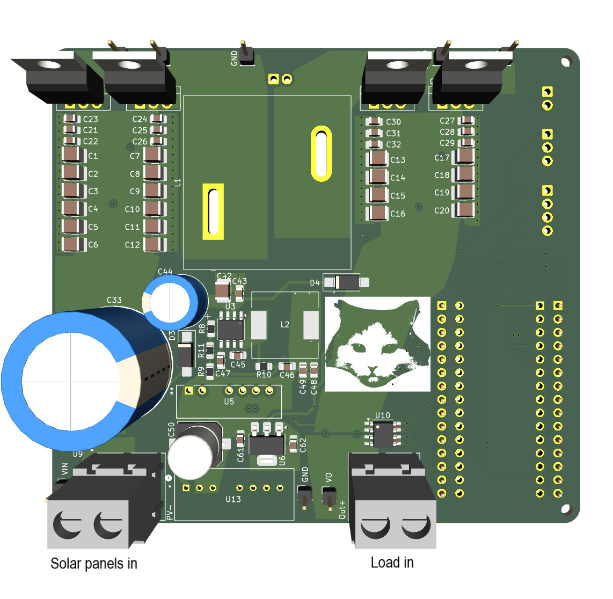
\includegraphics[width=0.95\linewidth]{pcb_top_components.png}
    \caption{PCB top view with components}
    \label{fig:pcb-top-components}
  \end{minipage}\hfill
  \begin{minipage}[t]{0.47\textwidth}
    \centering
    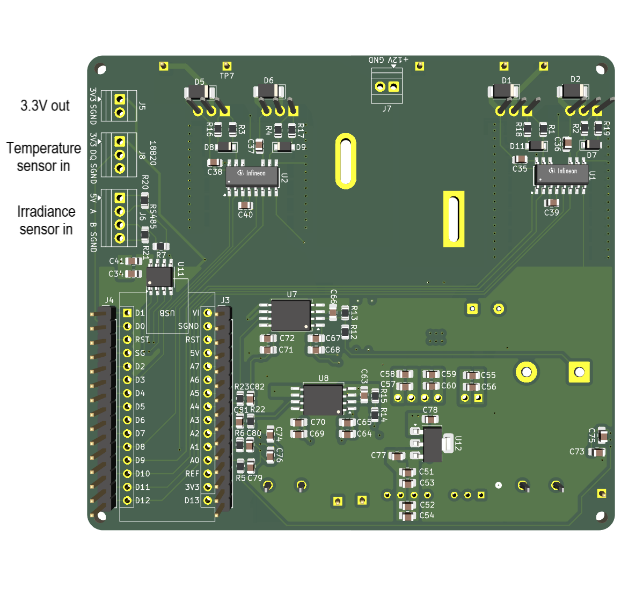
\includegraphics[width=0.95\linewidth]{pcb_bottom_components.png}
    \caption{PCB bottom view with components}
    \label{fig:pcb-bottom-components}
  \end{minipage}
\end{figure}

Connect the solar panels to the screw terminal labelled ``Solar panels in''. Connect the controlled output load or battery connection to the output/load terminals according to the practical instructions. 

\textit{Engineering Judgment:} Do not rely strictly on printed PCB labels for high-power connections. Always verify the polarity of your panels and batteries with a multimeter before plugging them in to avoid catastrophic reverse-polarity damage.

\section{STM32 Interface and CubeMX Configuration}
\label{sec:stm32-interface}

The board is designed for an STM32 NUCLEO-F303K8 microcontroller. The NUCLEO board plugs directly into the PCB headers. Table~\ref{tab:firmware-interface} gives the practical signal map that you need when configuring the firmware in CubeMX. 

\begin{table}[H]
  \centering
  \footnotesize
  \caption{STM32 pin and PCB signal map}
  \label{tab:firmware-interface}
  \begin{tabularx}{\textwidth}{@{}L{0.12\textwidth} L{0.21\textwidth} L{0.20\textwidth} Y@{}}
    \toprule
    \rowcolor{TableHead}\textbf{NUCLEO label} & \textbf{STM32 pin/function} & \textbf{PCB signal label} & \textbf{Purpose} \\
    \midrule
    D1  & PA9 / \code{TIM1\_CH2} & \code{BST\_LOPWM} & PWM signal for the boost-side low switch (SW3). \\
    D3  & PB0 / \code{TIM1\_CH2N} & \code{BST\_HIPWM} & PWM signal for the boost-side high switch (SW4). \\
    D9  & PA8 / \code{TIM1\_CH1} & \code{BCK\_HIPWM} & PWM signal for the buck-side high switch (SW1). \\
    D10 & PA11 / \code{TIM1\_CH1N} & \code{BCK\_LOPWM} & PWM signal for the buck-side low switch (SW2). \\
    D8  & PF1 / GPIO output & \code{BST\_DIS} & Active-high disable signal for the \href{https://www.infineon.com/part/2EDB8259Y}{Infineon 2EDB8259Y} boost-side gate driver. \\
    D11 & PB5 / GPIO output & \code{BCK\_DIS} & Active-high disable signal for the buck-side gate driver. \\
    D13 & PB3 / GPIO output & \code{BST\_STP} & Shoot-through or dead-time control signal for the boost side. \\
    D12 & PB4 / GPIO output & \code{BCK\_STP} & Shoot-through or dead-time control signal for the buck side. \\
    A0  & PA0 / \code{ADC1\_IN1} & \code{I\_IN} & ADC feedback for input/PV current. \\
    A1  & PA1 / \code{ADC1\_IN2} & \code{I\_O} & ADC feedback for output current. \\
    A3  & PA4 / \code{ADC2\_IN1} & \code{V\_O} & ADC feedback for output voltage. \\
    A4  & PA5 / \code{ADC2\_IN2} & \code{V\_IN} & ADC feedback for input/PV voltage. \\
    D0  & PA10 / GPIO one-wire & \code{DQ} & Bidirectional data line for the \href{https://www.analog.com/media/en/technical-documentation/data-sheets/ds18b20.pdf}{DS18B20 temperature sensor}. \\
    D4  & PB7 / UART RX & \code{RO} & Receive data from the \href{https://www.st.com/resource/en/datasheet/st4e1216.pdf}{ST4E1216IDT RS485 transceiver}. \\
    D5  & PB6 / UART TX & \code{DI} & Transmit data to the ST4E1216IDT RS485 transceiver. \\
    D6  & PB1 / GPIO output & \code{RE} & RS485 receiver enable, active low. \\
    D7  & PF0 / GPIO output & \code{DE} & RS485 driver enable, active high. \\
    \bottomrule
  \end{tabularx}
\end{table}

\begin{warnbox}{PWM pin verification required}
The official NUCLEO-F303K8 connector table maps D1 to PA9 and D3 to PB0. Therefore the boost-side D1/D3 channel labels must be checked against the actual PCB routing before energising the converter. Configure and probe the pins on an oscilloscope. If the observed high-side and low-side signals are reversed, correct the CubeMX mapping before continuing.

Furthermore, \textbf{Dead-Time is critical}. If the top and bottom MOSFETs turn on simultaneously, a shoot-through short circuit will occur. You must configure the STM32's Advanced Timer to insert approximately 100~ns of dead-time between complimentary channel switching states.
\end{warnbox}

\subsection{CubeMX peripheral checklist}

Configure the peripherals in a way that makes safe startup the default:
\begin{itemize}
  \item \textbf{Clock}: set a stable system clock and confirm timer clock frequency before calculating PWM period.
  \item \textbf{TIM1}: use PWM generation with complementary outputs; enable preload; configure dead time; do not start outputs until all safe-state GPIOs have been set.
  \item \textbf{ADC1 and ADC2}: configure the four analog channels; use sufficient sample time for stable sensor readings; use DMA if continuous sampling is required.
  \item \textbf{GPIO}: set disable pins (\code{BCK\_DIS}, \code{BST\_DIS}) high immediately upon boot to keep gate drivers disabled safely.
  \item \textbf{USART}: configure the irradiance UART for the sensor's Modbus-RTU settings.
  \item \textbf{Debug}: keep SWD enabled so the firmware can be stopped and inspected during bring-up.
\end{itemize}


\section{Voltage and Current Sensing}
\label{sec:sensing}

The STM32 does not measure panel voltage or current directly. It measures sensor output voltages between approximately $0$ and $3.3\,\mathrm{V}$. Firmware must convert ADC counts into engineering units before using them in MPPT or fault checks.

\subsection{ADC conversion}

For a 12-bit ADC with a reference voltage $\Vref$, the measured ADC input voltage is
\begin{equation}
  \Vadc = \frac{N}{4095}\Vref,
  \label{eq:adc-voltage}
\end{equation}
where $N$ is the raw ADC count. If the STM32 analog reference is $3.3\,\mathrm{V}$, then one count is approximately $0.806\,\mathrm{mV}$ at the ADC input.

\textit{Engineering Challenge:} ADC readings are inherently noisy due to 250~kHz switching transients. If you feed raw, noisy readings into your MPPT algorithm, it will behave erratically. You must research, design, and implement a digital filter (such as an Exponential Moving Average) in software to smooth the data.

\subsection{Voltage sensors}

Two \href{https://www.ti.com/product/AMC0311S}{TI AMC0311S} isolated amplifiers sense input and output voltages. The voltage divider feeds the isolated amplifier input, and the amplifier output is measured by the STM32 ADC. The circuit schematic is shown in Figure~\ref{fig:voltage-sensor}.

\begin{figure}[H]
  \centering
  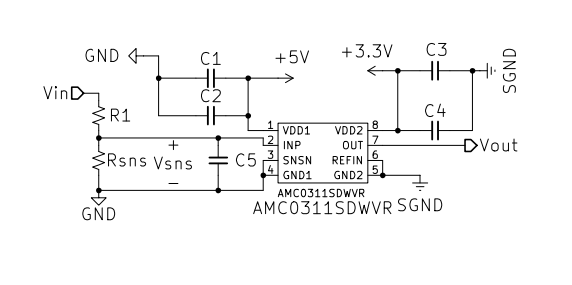
\includegraphics[width=0.70\textwidth]{amc0311s_voltage_sensor.png}
  \caption{AMC0311S voltage sensor}
  \label{fig:voltage-sensor}
\end{figure}

The input voltage sensor is connected to \code{ADC2\_IN2} on A4, and the output voltage sensor is connected to \code{ADC2\_IN1} on A3.

\begin{table}[H]
  \centering
  \caption{Voltage sensor parameter values}
  \label{tab:voltage-sensor-values}
  \begin{tabularx}{0.76\textwidth}{@{}Ycc@{}}
    \toprule
    \rowcolor{TableHead} & \textbf{Input voltage sensor} & \textbf{Output voltage sensor} \\
    \midrule
    \textbf{$R_1$ ($\mathrm{k}\Omega$)}        & 100 & 100 \\
    \textbf{$R_{\mathrm{sns}}$ ($\mathrm{k}\Omega$)} & 2.2 & 3.6 \\
    \bottomrule
  \end{tabularx}
\end{table}

Assuming unity gain from the AMC0311S signal path and the divider shown in Figure~\ref{fig:voltage-sensor}, the voltage before the divider is estimated from
\begin{equation}
  V_{\mathrm{meas}} = \Vadc \left(\frac{R_1+R_{\mathrm{sns}}}{R_{\mathrm{sns}}}\right).
  \label{eq:voltage-sensor}
\end{equation}

Using the resistor values in Table~\ref{tab:voltage-sensor-values}, the approximate scale factors are:
\begin{align}
  V_{\mathrm{in}}  &\approx \Vadc(46.45),\\
  V_{\mathrm{o}}   &\approx \Vadc(28.78).
\end{align}

\subsection{Current sensors}

Two \href{https://www.allegromicro.com/~/media/files/datasheets/CT416-datasheet.pdf}{Allegro CT416} magnetoresistive current sensors measure current. A CT416-HSN820DR unidirectional $20\,\mathrm{A}$ sensor is used for the input current, and a CT416-HSN830MR bidirectional $\pm30\,\mathrm{A}$ sensor is used for the output current. The input current sensor output is connected to \code{ADC1\_IN1} on A0. The output current sensor output is connected to \code{ADC1\_IN2} on A1.

\begin{figure}[H]
  \centering
  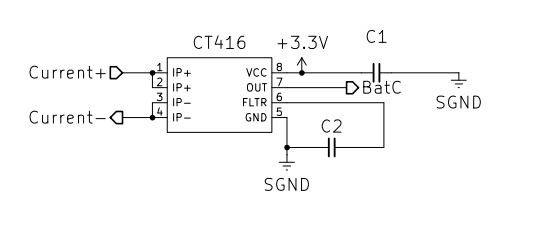
\includegraphics[width=0.62\textwidth]{ct416_current_sensor.png}
  \caption{CT416 current sensor}
  \label{fig:current-sensor}
\end{figure}

For the CT416-HSN820DR input-current sensor, the nominal sensitivity is $100\,\mathrm{mV/A}$. For a unidirectional sensor, the output is approximately
\begin{equation}
  \Iin \approx \frac{\Vadc - V_{\mathrm{offset,in}}}{0.100}.
\end{equation}
You will need to measure $V_{\mathrm{offset,in}}$ at zero current in your initialization code before using the reading.

For the CT416-HSN830MR output-current sensor, the nominal sensitivity is $33.3\,\mathrm{mV/A}$ and the zero-current output is near mid-supply. Estimate output current with
\begin{equation}
  \Iout \approx \frac{\Vadc - V_{\mathrm{offset,o}}}{0.0333}.
\end{equation}

\subsection{Power calculation}

The MPPT algorithm must use input-side PV power:
\begin{equation}
  \Pin = V_{\mathrm{in}} I_{\mathrm{in}}.
\end{equation}
Output voltage and output current are still important, but they are mainly used for battery/load monitoring, efficiency estimation, and fault detection. 


\section{Irradiance Sensor and RS485 Interface}

A \href{https://wiki.dfrobot.com/sen0640/docs/20430}{DFRobot SEN0640 photoelectric solar-radiation sensor} is provided for irradiance sensing. It can be plugged into screw terminal \code{J8}. The PCB uses an \href{https://www.st.com/resource/en/datasheet/st4e1216.pdf}{ST4E1216IDT RS485 transceiver} to convert between the differential RS485 bus and the STM32 UART pins.

The SEN0640 measures solar radiation over a 400--1100 nm wavelength range and reports values over \textbf{Modbus-RTU}. The default Modbus address is \code{0x01}. The default UART settings are 4800 bit/s, 8 data bits, no parity, and 1 stop bit.

\subsection{The Physical Layer: RS-485 Direction Control}

RS-485 uses differential wires to reject noise. However, it is \textbf{half-duplex}: it can only transmit OR receive at one time, not both. The STM32 must explicitly control whether the transceiver is listening or transmitting using the Driver Enable (\code{DE}) and Receiver Enable (\code{RE}) pins.
\begin{itemize}
  \item To \textbf{send} a request to the sensor: Set \code{DE}=1.
  \item To \textbf{listen} for the sensor's reply: Set \code{DE}=0 and \code{RE}=0.
\end{itemize}

\textit{The Gotcha:} If you pull \code{DE} low \textit{before} the STM32's UART has finished physically pushing the last bit out of the wire, your message will be corrupted. You must investigate the difference between the UART \code{TXE} (Transmit Data Register Empty) flag and the \code{TC} (Transmission Complete) flag in the STM32 HAL.

\subsection{The Protocol Layer: Modbus-RTU}

Modbus is a standardised way of formatting byte arrays. The sensor is the "Slave" (Address \code{0x01}) and the STM32 is the "Master". To read the current solar radiation value, send a Modbus function \code{0x03} request for register \code{0x0000} with length \code{0x0001}. 

For the default address, the request frame is:
\begin{lstlisting}[caption={SEN0640 read-irradiance request bytes}]
01 03 00 00 00 01 84 0A
\end{lstlisting}

A response carrying $100\,\mathrm{W/m^2}$ is:
\begin{lstlisting}[caption={Example SEN0640 response bytes}]
01 03 02 00 64 9B AF
\end{lstlisting}

\textbf{The Engineering Challenges:}
\begin{enumerate}
    \item \textbf{Endianness:} Modbus transmits data "Big-Endian" (most significant byte first). In the example above, \code{0x0064} equals 100. However, ARM Cortex-M processors (like your STM32) store data "Little-Endian". You will have to write code to swap the bytes when you receive the 16-bit irradiance value.
    \item \textbf{CRC Verification:} Modbus requires a Cyclic Redundancy Check (CRC-16) at the end of every message to verify data integrity (e.g., \code{9B AF}). You will need to implement a standard Modbus CRC-16 algorithm in C to verify incoming messages and validate your own outgoing requests.
\end{enumerate}


\section{Firmware Architecture}

When building power electronics, you \textbf{never} want to place all behaviour inside one large \code{while(1)} loop with hard-coded pin operations. You must implement the logic using a \textbf{State Machine}. Separate hardware drivers, measurement conversion, fault checks, and MPPT logic. 

\subsection{Main control-loop timing}

You have to juggle tasks at different speeds:
\begin{itemize}
  \item \textbf{250 kHz:} PWM generation (Hardware Timer).
  \item \textbf{Fast (~1-10 kHz):} ADC acquisition (commonly using DMA) and Fault checking.
  \item \textbf{Medium (~10-50 Hz):} MPPT update. Allow the converter and measurements to settle after changing the duty cycle.
  \item \textbf{Slow (~1 Hz):} Irradiance polling and PC Data Logging.
\end{itemize}

\textit{Data Logging Warning:} You need to send data to a computer over UART to save your results. Standard \code{printf()} over UART is extremely slow. If you call a blocking transmit function inside your main control loop, you will miss ADC measurements and potentially blow up the converter. Use non-blocking interrupts, DMA, or place your PC communication in a slow, strictly controlled timer block.

\subsection{State machine}

A suggested structure is shown in Table~\ref{tab:firmware-states}.

\begin{table}[H]
  \centering
  \caption{Suggested firmware states}
  \label{tab:firmware-states}
  \begin{tabularx}{\textwidth}{@{}L{0.18\textwidth} Y Y@{}}
    \toprule
    \rowcolor{TableHead}\textbf{State} & \textbf{Purpose} & \textbf{Exit condition} \\
    \midrule
    \code{INIT} & Configure peripherals and force safe outputs. & Initialisation complete. \\
    \code{IDLE} & PWM stopped, gate drivers disabled, measurements active. & User/test command and valid measurements. \\
    \code{STARTUP} & Apply approved precharge/startup sequence and small duty command. & Voltages/currents plausible and stable. \\
    \code{RUN} & Execute MPPT, update duty cycles, log data. & Fault, stop command, or test complete. \\
    \code{FAULT} & Disable switching and record cause. & Manual reset or approved recovery condition. \\
    \bottomrule
  \end{tabularx}
\end{table}

\subsection{Guided MPPT and PSO pseudocode}

Particle swarm optimisation (PSO) can be used by treating each particle as a candidate converter command. The candidate may be a buck duty cycle, a boost duty cycle, or a mapped operating variable. Each particle stores its current position, velocity, personal best position, and personal best measured power.

This pseudocode provides a conceptual framework. You must determine the exact PSO coefficients and algorithm integration according to the practical instructions.

\begin{lstlisting}[caption={Guided PSO-style MPPT structure}]
initialise_particles_with_safe_duty_values();
global_best = first_valid_particle();

while (state == RUN) {
    read_and_filter_measurements();
    
    // Hardware limits must override the algorithm!
    check_fault_limits();
    if (fault_active) {
        disable_pwm_and_enter_fault();
        break;
    }

    particle = select_next_particle();
    
    // Never allow the optimiser to bypass safe duty clamps
    duty = clamp(particle.position, DUTY_MIN, DUTY_MAX);
    ramp_pwm_to(duty);
    wait_for_converter_to_settle();

    read_and_filter_measurements();
    p_pv = v_in * i_in;

    if (p_pv > particle.best_power) {
        particle.best_power = p_pv;
        particle.best_position = particle.position;
    }

    if (p_pv > global_best.power) {
        global_best.power = p_pv;
        global_best.position = particle.position;
    }

    update_particle_velocity_and_position(
        particle,
        particle.best_position,
        global_best.position);
}
\end{lstlisting}

\subsection{Fault handling}

When a fault occurs:
\begin{enumerate}
  \item immediately command zero or safe PWM compare values;
  \item assert \code{BCK\_DIS} and \code{BST\_DIS} to disable gate drivers;
  \item stop MPPT updates;
  \item record the fault source, latest measurements, and duty command;
  \item require a deliberate reset or approved recovery action before re-enabling switching.
\end{enumerate}




\section{Troubleshooting}

\begin{table}[H]
  \centering
  \caption{Common faults and first checks}
  \label{tab:troubleshooting}
  \begin{tabularx}{\textwidth}{@{}L{0.24\textwidth} Y Y@{}}
    \toprule
    \rowcolor{TableHead}\textbf{Symptom} & \textbf{Likely causes} & \textbf{First checks} \\
    \midrule
    No PWM on a pin & Timer not started, wrong alternate function, GPIO still configured as output/input & Check CubeMX pin mode, start calls, and oscilloscope ground. \\
    Complementary pair overlaps & Dead time missing or wrong channel pairing & Recheck TIM1 complementary-output settings and D1/D3 mapping. \\
    Gate driver does not switch & Disable pin high, supply missing, wrong PWM input & Measure \code{DIS}, driver supply, and input pin waveform. \\
    ADC value stuck & Wrong ADC channel, pin not analog, DMA not started & Check CubeMX ADC rank/channel and raw counts. \\
    Current nonzero at no load & Sensor offset not calibrated, noise, wrong sign convention & Record zero-current offset and apply filtering. \\
    Irradiance timeout & RS485 direction wrong, A/B reversed, baud mismatch, wrong CRC & Check \code{DE}/\code{RE}, UART settings, and request bytes. \\
    MPPT unstable & Update too fast, duty step too large, insufficient filtering, weak fault limits & Slow the MPPT loop, ramp duty, and log each candidate. \\
    Output voltage rises too high & Load disconnected, duty too high, wrong mode transition & Disable PWM and inspect load, limits, and duty clamp. \\
    \bottomrule
  \end{tabularx}
\end{table}

\section{Reference Resources}
\label{sec:resources}

Use the following references when configuring firmware, implementing algorithms, or checking component behaviour:
\begin{itemize}
  \item \href{https://www.st.com/en/development-tools/stm32cubeide}{STM32CubeIDE download page}.
  \item \href{https://www.youtube.com/watch?v=FAb4DnOZ9LA}{Introductory STM32CubeIDE and CubeMX setup video for getting started}.
  \item \href{https://www.st.com/en/evaluation-tools/nucleo-f303k8.html}{NUCLEO-F303K8 product page}.
  \item \href{https://www.st.com/resource/en/user_manual/um1956-stm32-nucleo32-boards-mb1180-stmicroelectronics.pdf}{UM1956 STM32 Nucleo-32 boards user manual}.
  \item \href{https://www.st.com/en/microcontrollers-microprocessors/stm32f303/documentation.html}{STM32F303 documentation page}.
  \item \href{https://www.st.com/resource/en/datasheet/stm32f303c6.pdf}{STM32F303x6/x8 datasheet}.
  \item \href{https://www.st.com/resource/en/reference_manual/rm0316-stm32f303xbcde-stm32f303x68-stm32f328x8-stm32f358xc-stm32f398xe-advanced-armbased-mcus-stmicroelectronics.pdf}{RM0316 STM32F303 reference manual for peripheral setup}.
  \item \href{https://www.infineon.com/part/2EDB8259Y}{Infineon 2EDB8259Y gate-driver page}.
  \item \href{https://www.ti.com/product/AMC0311S}{TI AMC0311S isolated-amplifier page}.
  \item \href{https://www.allegromicro.com/~/media/files/datasheets/CT416-datasheet.pdf}{Allegro CT416 current-sensor datasheet}.
  \item \href{https://www.analog.com/media/en/technical-documentation/data-sheets/ds18b20.pdf}{Analog Devices DS18B20 temperature-sensor datasheet}.
  \item \href{https://www.st.com/resource/en/datasheet/st4e1216.pdf}{ST4E1216 RS485 transceiver datasheet}.
  \item \href{https://www.csimn.com/CSI_pages/Modbus101.html}{Control Solutions Modbus protocol tutorial}.
  \item \href{https://wiki.dfrobot.com/sen0640/docs/20430}{DFRobot SEN0640 Modbus-RTU reference}.
  \item \href{https://www.offgridtec.com/media/product_attachements/YingliSolar_410W\%20YLM-J\%203.0\%20PRO_Datasheet.pdf}{Yingli YLM-J 3.0 PRO panel datasheet}.
\end{itemize}

\end{document}
